\section{Material and methods}
This research was conducted under approval from the University of Sydney Human Research Ethics Committee, HREC 2014/557.
\subsection{Participants}
Structural (T1-weighted) MR brain images were obtained (N = 313) from pre-existing MRI studies conducted at two different sites (site A and site B). The cohort from each site contained two diagnostic groups (schizophrenia and healthy adults), however these groups were not evenly distributed over sites (see Table \ref{tab:cohort}). All clinical cases met DSM-IV criteria for their disorder with no other Axis I disorders, on the basis of either the Mini-International Neuropsychiatric Interview \citep{hergueta1998mini} or the Structured Clinical Interview for DSM-IV Axis I and II Disorders \citep{first2002structured}. Participants were aged 18-65 years and spoke fluent English. Exclusion criteria included the presence of an organic brain disorder, brain injury with post-traumatic amnesia, mental retardation (WAIS-III IQ score less than 80), movement disorders and recent (within 6 months) substance dependence or electroconvulsive therapy. Healthy adults were also screened for the absence of personal or family history of any DSM-IV Axis I disorder.

\begin{table}[htbp]
  \centering
  \caption{Subject and gender distribution across sites (m:male, f:female)}
    \begin{tabular}{l|lll}
    \toprule
     & \textbf{Site A} & \textbf{Site B} &\textbf{Total} \\
    \midrule
    Control \\
    \hspace{1em}n &41 &101 &142 \\
    \hspace{1em}age $\pm$ SD    &29.7$\pm$13.1 &31.2$\pm$8.7 & 31.2$\pm$10.1	  \\
    \hspace{1em}m/f   & 23/18 & 52/49 & 75/67\\
     Schizophrenia\\
     \hspace{1em}n &17 &154 &171 \\
     \hspace{1em}age $\pm$ SD    &44.8$\pm$11.1 &38.0$\pm$9.5	 & 38.7$\pm$9.8  \\
     \hspace{1em}m/f   & 7/10 & 57/97 & 64/107\\
     %Bipolar \\
     %\hspace{1em}age $\pm$ SD    &  24.5$\pm$5.4&43.3$\pm$11.4& 34.5$\pm$13.1 	  \\
    %\hspace{1em}m/f   & 12/9 & 12/12 & 24/21\\
     Total \\
     \hspace{1em}n &58 &255 &313 \\
     \hspace{1em}age $\pm$ SD    & 34.1$\pm$14.1&	35.3$\pm$9.7 & 35.1$\pm$10.7\\
    \hspace{1em}m/f   & 30/28 & 109/158 & 139/174\\
    \bottomrule
    \end{tabular}%
  \label{tab:cohort}%
\end{table}

\subsection{MR Scanner, image data and preprocessing}
Data were collected from two different MRI sites: Site A hosted a Phillips Achieva 3T with a 8-channel headcoil and receiver (NeuRA, Randwick NSW, Australia); and Site B hosted a GE Discovery MR750 3T with a 8-channel headcoil and receiver (Brain and Mind Centre, Camperdown NSW, Australia). T1-weighted image volumes were acquired using a standard but scanner-specific MPRAGE acquisition sequence. T1 images from Site A were acquired with a 3D Fast Spoiled Gradient Recall Echo (FSPGR) sequence with SENSE acceleration; 8.3-ms TR, 3.2-ms TE; and 11 degree flip angle, and comprised of 180 sagittal 1-mm slices in a 256 x 256 matrix (1 mm isotropic voxel dimensions). Images from Site B were acquired with a 3D Turbo Field Echo sequence (TFE) with ASSET acceleration; 7.192-ms TR, 2.732-ms TE; and 12 degree flip angle, and comprised of 176 sagittal 1-mm slices in a 256 x 256 matrix (1 mm isotropic voxel dimensions).

%  according to a widely adopted procedure described in Ashburner (2010, "optimized VBM").
Image preprocessing was designed to remove as much of the site differences as possible given standard tools available, before applying the novel GAN method described in the next section. All preprocessing occurred in SPM12 (http://www.fil.ion.ucl.ac.uk/spm), running under Matlab 8.4 (Math Works, Natick, MA, USA). After checking for scanner artifacts and gross anatomical abnormalities for each image, we reoriented the original images along the anterior-posterior commissure (AC-PC) line and set the AC as the origin of the spatial coordinates to assist the normalization algorithm. The unified segmentation procedure in SPM12 was used to segment all the images into mean corrected gray matter (GM), white matter (WM) and cerebrospinal fluid (CSF) space, i.e. maps of probability values representing the probability of a voxel containing a specific tissue type. Mean correction was applied to remove site differences in the bias field. A fast diffeomorphic image registration algorithm \citep{ashburner2007fast} was used to warp the GM partitions into a new study-specific reference space representing an average of all 313 subjects included in the analysis. As an initial step, a set of study-specific templates and the corresponding deformation fields, required to warp the data from each subject to the new reference space, were created using the GM partitions \citep{ashburner2009computing}. Each subject-specific deformation field was used to warp the corresponding GM partition into the new reference space with the aim of maximizing accuracy and sensitivity \citep{yassa2009quantitative}; the warped GM partitions were affine transformed into the MNI space and an additional `modulation' step was used to scale the GM probability values by the Jacobian determinants of the deformations in order to ensure that the total amount of gray matter in each voxel was conserved after the registration \citep{ashburner2000voxel,good2001cerebral,mechelli2005structural}. After this preprocessing, we obtained bias-field corrected, modulated, normalized gray matter density maps, from which we extracted the middle five 2D sagittal slices to be used to train the GAN model described below.

\subsection{Generative Adversarial Networks}
Rather than removing any remaining scanner artifacts and biases from the images, we seek to transform one set of images from a site to images that come from the distribution of images from the other site, while still preserving the important features of the original images.

\textbf{Notation}: In the following, we have defined capital bold font, $\mathbf{X}$, as a matrix or a set of images and lower case bold font, $\mathbf{x}$, as a vector or one example image. $G_\mathbf{\theta}$, $D_\mathbf{\phi}$ denotes a mapping function parameterised by $\mathbf{\theta}$ and $\mathbf{\phi}$, respectively. $P(\mathbf{X})$ indicates the probability distribution for the imaging set $\mathbf{X}$, and $\hat{P}(\mathbf{X})$ is an estimate of that probability distribution.

The problem at hand can be described as image-to-image translation in the computer vision literature where the goal is to learn a mapping function between a set of MRI images from domain $\mathbf{X}$ and another set of images from domain $\mathbf{Y}$; learn $G: \mathbf{X}\rightarrow \mathbf{Y}$ such that $G(\mathbf{x})$ for each $\mathbf{x} \in \mathbf{X}$ is indistinguishable from the set of images from domain $\mathbf{Y}$.

The CycleGAN \citep{zhu2017unpaired} and DiscoGAN \citep{kim2017learning} have been developed to learn cross domain relationships between sets of natural objects such as from horses to zebras, edges to photos and Monet artworks to realistic photos. The advantage of these models is that they do not require paired sets of training samples, $\{\mathbf{x}_i,\mathbf{y}_i\}^N_{i=1}$, which is often difficult to obtain for neuro-imaging data, and instead only require unpaired imaging data consisting of a source set $\{\mathbf{x}_i\}^N_{i=1}\in \mathbf{X}$ and target set $\{\mathbf{y}_j\}^M_{j=1} \in \mathbf{Y}$ , without any $\mathbf{x}_i$'s necessarily corresponding to any $\mathbf{y}_j$'s. These models attempt to transform the underlying distribution of $P(\mathbf{X})$ to an estimate of $P(\mathbf{Y})$, $\hat{P}(\mathbf{Y})$, through $G$ while still preserving the important features of the original sample, $\mathbf{x}_i$, but also merging these with the particular characteristics of $P(\mathbf{Y})$.

To learn this mapping function, an adversarial training regime was utilised using the GAN formulation. The generator, $G_\mathbf{\theta}$, represented as a convolutional neural network defined by parameters $\mathbf{\theta}$, takes as input, images from $\mathbf{X}$ and transforms these images, $G_\mathbf{\theta}(\mathbf{x})$, as if they were sampled from $P(\mathbf{Y})$. The discriminator, $D_\mathbf{\phi}$ on the other hand, is a supervised classifier represented as a convolutional neural network. The discriminator observes two inputs, the observed images from $\mathbf{Y}$ and generated samples $G_\mathbf{\theta}(\mathbf{x})$. The goal of the discriminator is to output a probability that its inputs are either real or fake, with the true labels being observed samples as real and generated samples as fake. The discriminator attempts to learn that its output from samples of $\mathbf{Y}$,  $D_\mathbf{\phi}(\mathbf{y})$, are given to be given values near 1 and inputs from the generator, $D_\mathbf{\phi}(G_\mathbf{\theta}(\mathbf{x}))$, to be values close to 0. However, at the same time, the generator will attempt to make the quantity, $D_\mathbf{\phi}(G_\mathbf{\theta}(\mathbf{x}))$ to approach 1. At equilibrium, $D_\mathbf{\phi}(\mathbf{y})=\frac{1}{2}$ for all $\mathbf{y}$ and $G_\mathbf{\theta}(\mathbf{x})$ which means that the discriminator is unable to distinguish between real and generated samples.

The generator and discriminator face two competing objectives during training; the discriminator attempts to push $D_\mathbf{\phi}(G_\mathbf{\theta}(\mathbf{x}))$ to 0 and whilst on the other hand, the generators strives to fool the discriminator and make $D_\mathbf{\phi}(G_\mathbf{\theta}(\mathbf{x}))$ equal to 1.

More specifically, the Least Squares GAN (LSGAN) \citep{mao2016least} is used to train the discriminator and generator, where the discriminator's objective function is
\begin{equation}
	\label{eqn:discrim_loss}
    \min_\mathbf{\phi} \frac{1}{2}E_{\mathbf{y}\sim p(\mathbf{Y})}[(D_\mathbf{\phi} (\mathbf{y}) - 1)^2] + \frac{1}{2}E_{\mathbf{x}\sim p(\mathbf{X})}[(D_\mathbf{\phi} (G_\mathbf{\theta}(\mathbf{x})))^2],
\end{equation}
and the generator competes against the discriminator by having the objective function
\begin{equation}
	\label{eqn:gen_loss}
    \min_\mathbf{\theta} \frac{1}{2}E_{\mathbf{x}\sim p(\mathbf{X})}[(D_\mathbf{\phi} (G_\mathbf{\theta}(\mathbf{x}))-1)^2].
\end{equation}
Equation \ref{eqn:discrim_loss} and \ref{eqn:gen_loss} is typically optimised using stochastic gradient decent where $\mathbf{\phi}$ is updated keeping the generator's parameters fixed for one or more iterations and vice versa. Details about the training parameters are described in Section \ref{implementation}.  Equation \ref{eqn:discrim_loss} is optimised in a supervised manner where the ground truth labels, real or fake, are provided to the discriminator through the inputs $\mathbf{y}$ and $G_\mathbf{\theta}(\mathbf{x})$ respectively. Mao et al. demonstrated that minimising the objective function of LSGAN yields minimising the Pearson $\chi^2$ divergence between $\mathbf{Y}$ and $G_\mathbf{\theta}(\mathbf{x})$ \citep{mao2016least}.

\begin{comment}
The discriminator learns a decision boundary between real and fake samples and although some fake samples might be correctly classified, Equation \ref{eqn:discrim_loss} penalises samples further away from the decision boundary. Since $\mathbf{\phi}$ is fixed when updating the generator, the the decision boundary learned by the discriminator is also kept fixed. The dependence between the generator on the discriminator for learning (Equation \ref{eqn:gen_loss}) encourages the generator to produce samples closer to the decision boundary. On the next iteration, this causes the discriminator to update its decision boundary closer to the real data's manifold. The process repeats, making the decision boundary to pass through the real data manifold and the generated samples closer to the manifold of real data.
\end{comment}

Equation \ref{eqn:gen_loss}, in contrast to the learning objective of the discriminator, shows the generator does not have the same level of supervision as the discriminator. While although they have competing objectives, the generator improves its generation of samples, not because of the directive by a supervisor but rather, by the information provided by the discriminator. It is through the cooperation between the generator and discriminator that the generator learns the mapping function in an unsupervised manner. This enables the ability to learn the transformation that is data driven and without any a-priori knowledge of the processes that generated the two image sets.

The GAN objectives is not limited to Equations \ref{eqn:discrim_loss} and \ref{eqn:gen_loss}. Other adversarial formulations have been developed in order to minimise other divergence measures between the observed distribution and generated distribution such as the $f$-divergence \citep{nowozin2016f}, Jensen-Shannon divergence \citep{goodfellow2016nips} or other distance metrics to have different geometric interpretations such as, and not limited to, Earth Mover distance \citep{arjovsky2017wasserstein} and Integral Probability Metrics \citep{mroueh2017mcgan}.
Results based on the $f$-divergence, Jensen-Shannon divergence and Earth Mover distance were also included in experiments but produced similar results to the LSGAN. They have not been included for the sake of brevity.

\subsubsection{Cycle loss}
However, the transformation $G:\mathbf{X}\rightarrow \mathbf{Y}$ is ill-posed as there are infinitely many mappings, $G(\mathbf{x})$, that could induce the estimated distribution $\hat{P}({\mathbf{Y}})$. This means that each $\mathbf{x}$ and output $G(\mathbf{x})$ do not necessarily have to have any meaningful relationship.  For example, a possible outcome is that $G_\mathbf{\theta}$ learns to transform all $\mathbf{x} \in \mathbf{X}$ , to only one particular example of $\mathbf{Y}$. This outcome is known as mode collapse where the generator learns to map several different input values to the same output point that fools the discriminator and the model is unable to make any progress in training.

To prevent this issue from occurring, the model is required to be constrained to a one-to-one correspondence (bijective mapping) by introducing the idea of a \textit{cycle} loss \citep{zhu2017unpaired}. If we have a mapping $G: \mathbf{X}\rightarrow \mathbf{Y}$ and another mapping $F: \mathbf{Y}\rightarrow \mathbf{X}$ then $G$ and $F$ should be inverses of each other. To ensure this, the generators $G$ and  $F$ are both trained simultaneously with their own adversarial loss and own parameters, $\mathbf{\theta_1}$ and $\mathbf{\theta_2}$ respectively but also adding a loss that encourages $F_\mathbf{\theta_2}(G_\mathbf{\theta_1}(\mathbf{x})) \approx \mathbf{x}$ and $G_\mathbf{\theta_1}(F_\mathbf{\theta_2}(\mathbf{y})) \approx \mathbf{y}$. The generators $G_\mathbf{\theta_1}$ and $F_\mathbf{\theta_2}$ are able to reconstruct the original set of images. Any distance metric function (L$_1$, Huber loss, cosine) could be used but in particular, the L$_2$ norm was used,
\begin{equation}
    \label{eqn: reconstuction_loss}
    L_{cycle}(G, F) =E_{\mathbf{x}\sim p(\mathbf{X})} [\| F_\mathbf{\theta_2}(G_\mathbf{\theta_1}(\mathbf{x})) - \mathbf{x}\|_2] +E_{\mathbf{y}\sim p(\mathbf{Y})} [\| G_\mathbf{\theta_1}(F_\mathbf{\theta_2}(\mathbf{y})) - \mathbf{y}\|_2].
\end{equation}
\begin{figure}[htp]
\begin{center}
 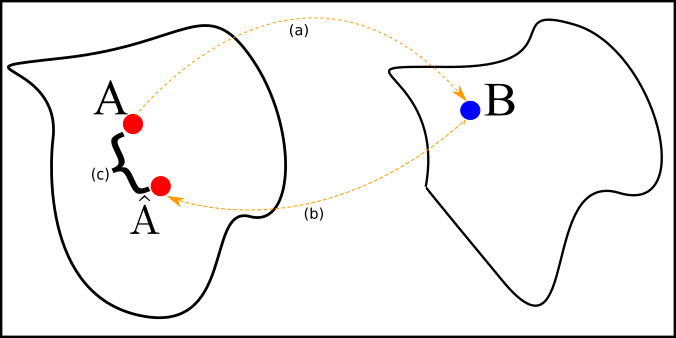
\includegraphics[width = 0.7\textwidth]{drawing.png}
    \end{center}
  \caption{\textbf{(a)}: Image A is mapped into the manifold of scanner set B through a a convolutional neural network (generator). \textbf{(b)}: This image is then transformed back to the original manifold to reconstruct the original image using a different CNN. \textbf{(c)}: The original and reconstructed image is compared using some distance metric (e.g. L$_1$ or L$_2$-norm).}
  \label{fig:pca_tsne}
\end{figure}
\subsubsection{Full objective}
The model contains two pairs of GANs, with each generator learning the respective mapping functions $G: \mathbf{X}\rightarrow \mathbf{Y}$ and $F: \mathbf{Y}\rightarrow \mathbf{X}$. Each generator will have their respective discriminators, $D_\mathbf{\phi_1}$ and $D_\mathbf{\phi_2}$, where $D_\mathbf{\phi_1}$ will discriminate between $\mathbf{x} \in \mathbf{X}$ and samples from $F_\mathbf{\theta_2}$ and conversely, $D_\mathbf{\phi_2}$ will distinguish between $\mathbf{y} \in \mathbf{Y}$ and the output of $G_\mathbf{\theta_1}$. The objective function of $G_\mathbf{\theta_1}$ and $D_\mathbf{\phi_2}$ is given respectively as
\begin{equation}
\label{eqn:full_eqn}
   \min_\mathbf{\theta_1} E_{\mathbf{x}\sim p(\mathbf{X})}[(D_\mathbf{\phi_2} (G_\mathbf{\theta_1}(\mathbf{x}))-1)^2] + \lambda L_{cycle}(G_\mathbf{\theta_1}, F_\mathbf{\theta_2})
\end{equation}
\begin{equation}
    \min_\mathbf{\phi_2} E_{\mathbf{y}\sim p(\mathbf{Y})}[(D_\mathbf{\phi_2} (\mathbf{y}) - 1)^2] + E_{\mathbf{x}\sim p(\mathbf{X})}[(D_\mathbf{\phi_2} (G_\mathbf{\theta_1}(\mathbf{x})))^2]
\end{equation}
where $\lambda$ is a constant that controls the relative importance between the adversarial loss and reconstruction loss.
The objective function for $F_\mathbf{\theta_2}$ and $D_\mathbf{\phi_1}$ are similarly defined.

\begin{comment}
\begin{figure}[htp]
\begin{center}
 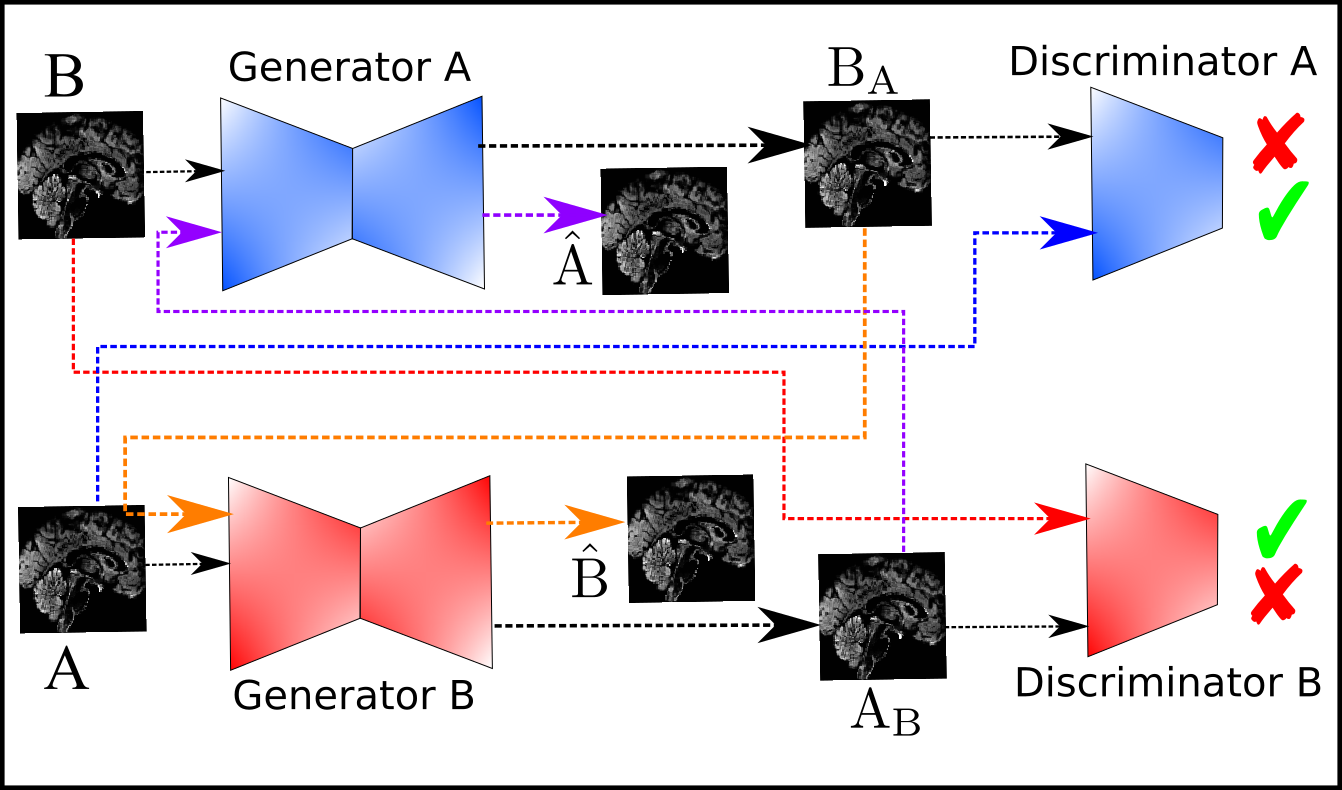
\includegraphics[width = 0.9\textwidth]{cycle_set.png}
    \end{center}
  \caption{Generator A takes an image scan from scanner B and transforms that image into another, $\textbf{B}_\textbf{A}$, such that Discriminator A cannot distinguish it from an image from scanner A. Generator B then takes $\textbf{B}_\textbf{A}$ in order to reconstruct the original image. This process is mirrored for image scans from scanner A.}
  \label{fig:cycle_diagram}
\end{figure}
\end{comment}

\subsection{Implementation} \label{implementation}
The generators and discriminators are fully convolutional neural networks. The discriminators are composed of six convolutional layers to create a receptive field of 30$\times$30 patches that aims to classify whether 30$\times$30 overlapping image patches are either real of fake. The transformations of the input consists of a succession of spatial 2D convolutions, a transformation that keeps the input distribution of each hidden layer similar during training by normalising a training batch (batch normalisation) and a voxel-wise non-linear transformation (also known as an activation function) of the results of the convolutions.

During training, the input distribution of each hidden layer may change after several iterations, known as internal covariate shift, due to the complicated non-linearities of the incoming neurons. The current hidden layers will have to continually adapt to these changes in the input distribution hence could slow down convergence. Batch normalisations attempts to rectify this by normalising the inputs to each hidden layer so that their distribution during training remains fairly constant \citep{DBLP:journals/corr/IoffeS15} which improves convergence of training. In regards to the choice of activation function, the \textit{leakyReLU} activation function was used as it was found to have the best qualitative performance except in the last layer of the discriminators where no activation function was used.

The generators contain two convolutional down sampling layers, reducing the dimensionality of the image by a factor of four, followed by six residual blocks to create new features of the data then another two convolutional upsampling layers to restore the image back to the original input dimensions. The residual blocks is composed of two convolutional layers that includes a `skip' connection, where the input to these layers are added to the output of the convolution layers. The residual blocks are critical to the generator as some portions of the image may not necessarily require any transformations. Therefore, including these residual layers will give the option of the network to skip convolutional layers and not undergo any change. Much like the discriminator, each convolutional layer is followed by batch normalisation and then a \textit{leakyReLU} activation function. However, the last layer of the generator uses a \textit{tanh} function that scales the output from -1 to 1, producing a new grey matter voxel map. More specific details about the architecture used is found in Table \ref{tab:network_arch}.

\begin{table}[htbp]
  \centering
  \begin{subtable}{\linewidth}
  \caption{Architecture of Generator}
    \begin{tabular}{c|ccccc}
    \toprule
    \textbf{Layer} & \textbf{Layer Type} & \textbf{No. of Filters} & \textbf{Stride}&  \textbf{Batch Norm} &\textbf{Activation Function} \\
    \midrule
    1    & Convolution	 & 32& 2 & No& LeakyReLU \\
    2    & Convolution & 64 & 2  & Yes& LeakyReLU \\
    3    & Convolution & 128 & 2 &  Yes &LeakyReLU  \\
    4-6    & Residual Block & 128 & 1 & Yes & LeakyReLU \\
    7    & Convolution Transpose & 64 & 2& Yes  & LeakyReLU\\
    8    & Convolution Transpose & 32 & 2 & Yes & LeakyReLU\\
    9    & Convolution & 1 & 1  & No & Tanh\\
    \bottomrule
    \end{tabular}%
  \label{tab:generator_arichitecture}%
  \end{subtable}
    \begin{subtable}{\linewidth}
  \caption{Architecture of Discriminator}
    \begin{tabular}{c|ccccc}
    \toprule
    \textbf{Layer} & \textbf{Layer Type} & \textbf{No. of Filters} & \textbf{Stride}&  \textbf{Batch Norm} &\textbf{Activation Function} \\
    \midrule
    1    & Convolution	 & 32& 2 & No& LeakyReLU \\
    2    & Convolution & 64 & 2  & Yes& LeakyReLU \\
    3    & Convolution & 128 & 2 &  Yes &LeakyReLU  \\
    4    & Convolution  & 128 & 1& Yes  & LeakyReLU\\
    5    & Convolution & 128 & 1 & Yes & LeakyReLU\\
    6    & Convolution & 1 & 1  & No & None\\
    \bottomrule
    \end{tabular}%
  \label{tab:discriminator_arichitecture}%
  \end{subtable}%
  \caption{Architecture of Generative Neural Network}
  \label{tab:network_arch}%
\end{table}%

During training, mini-batches consisting of eight sagittal slices were constructed from each scanner set. The filters of the CNN were intialised as described by Glorot and Bengio \citep{glorot2010understanding}. The network was trained using Adam optimisation \citep{kingma2014adam} with a starting learning rate of 2e-4 for the generators and discriminators. The generators and discriminators were trained concurrently; every one gradient step of the generator was taken with the discriminator parameters fixed followed by a gradient step of the discriminator, keeping the generator parameters fixed. Training was stopped when the cycle loss (Equation \ref{eqn: reconstuction_loss}) failed to stop decreasing. It was found empirically that the hyperparamter, $\lambda$, in Equation \ref{eqn:full_eqn} was set to $\lambda = 0.2$, balancing between faster convergence and qualitative results.

\subsection{Postprocessing}
For better classification results as outlined in Section \ref{evaluation_methods}, Principal Component Analysis (PCA) was used to transform the data into orthogonal eigenvector components, ordered according to their contribution of variation in explaining the dataset. The first 50 components was used as features to train the supervised learning models.

\subsection{Regression based correction methods}
The performance of the GAN correction was compared against two other popular \textit{post-hoc} correction methods: linear regression and Gaussian Process (GP) regression, which have previously been used to compensate for non-disease specific effects \citep{kostro2014correction,rao2017predictive, dukart2011age}.

A regression model was learned to estimate the GM density for every voxel based on examples of subject-specific covariate and their corresponding GM density maps. The general linear model for the voxels is given as
\begin{equation}
\mathbf{y} = \beta_0 + \mathbf{X}\mathbf{\beta} + \mathbf{\epsilon}, \epsilon\sim\mathcal{N}(0,\sigma^2),
\end{equation}
where $\mathbf{y}$ is a $N\times v$ matrix, where the columns represent the observed GM concentrations of each voxels and the rows are the observations of each of the $N$ control subjects. $\mathbf{X} \in \mathbb{R}^{N\times2}$ is the design matrix representing the subjects' scanner characteristic, coded as $\{0,1\}$ and the intercept term. $\mathbf{\beta}\in\mathbb{R}^{2\times v}$ represents the effect strengths associated to the scanner for each voxel and the coefficient of the intercept. The regression parameters $\mathbf{\beta}$ were estimated for each voxel independently with only the control subjects to avoid the confounding of disease. The model was applied to new data, $\mathbf{x}^{(*)}$, to obtain a subject specific template, and was subtracted from the observed GM map to get a corrected image.
\begin{equation}
\label{eqn:linear_regression_corr}
\hat{\mathbf{y}}_{OLS}^{(*)} = \mathbf{y}^{(*)} - \mathbf{x}^{(*)}\hat{\mathbf{\beta}}.
\end{equation}
where $\hat{\mathbf{y}}_{OLS}^{(*)}$ is the corrected GM map of the original, $\mathbf{y}^{(*)}$ of the test example.

The GP regression correction method is analogous to Equation \ref{eqn:linear_regression_corr}.
\begin{equation}
\label{eqn:gp_regression_corr}
\hat{\mathbf{y}}_{GPR}^{(*)} = \mathbf{y}^{(*)} - (\mathbf{k}_{\mathbf{\theta}}^{(*)})^T\mathbf{K}^{-1}_\mathbf{\theta}\mathbf{y}.
\end{equation}
$\hat{\mathbf{y}}_{GPR}^{(*)}$ and  $\mathbf{y}^{(*)}$ are the corrected and original images respectively. $\mathbf{K}_\mathbf{\theta}$ is the covariance kernel matrix of the training examples with the elements corresponding to the output of the kernel function $k_\mathbf{\theta}(\mathbf{x}_i,\mathbf{x}_j)$, for $i,j \in \{1,...,N\}$. The coefficients of the regression, $\mathbf{k}_{\mathbf{\theta}}^{(*)}$, is the kernel function values of the test example with all the training examples. The kernel used was similar to \cite{kostro2014correction} where the covariance between the input images $\mathbf{x}_i$ and $\mathbf{x}_j$ was
\begin{equation}
	k_{\mathbf{\theta},\sigma}(\mathbf{x}_i,\mathbf{x}_j) = \theta_1^2 \exp(-\theta_2^2(\mathbf{x}_i -\mathbf{x}_j)^2) + \theta_3^2 + \theta_4^2(\mathbf{x}_i)^T\mathbf{x}_j + \sigma^2\delta_{ij},
\end{equation}
where $\theta_k,k=\{1,...,4\}$ and $\sigma$ are scalar model hyperparameters, and $\delta_{ij}$ is the delta function; one if $i=j$ and zero, otherwise. The optimal hyperparameters were determined by maximising the likelihood function.
\subsection{Support vector machine classification}
Each correction method in this report (GAN, GP regression, linear regression) was evaluated by the improvement of a learned supervised classifier in a range of problems such as scanner, gender and disease classification. This evaluation method was used because of the lack of ground truth; there were a limited number of subjects who were scanned across the two centers in similar conditions (\textit{n} = 11, see Experiment 4: Reconstruction), which was insufficient to fully appraise our correction methods. A popular technique for the classification of high dimensional neuroimaging data is the support vector machine (SVM). It has been used for classification of many neurological diseases such as Alzheimer's Disease \citep{magnin2009support, jongkreangkrai2016computer}, Huntington's Disease \citep{kostro2014correction} and schizophrenia \citep{winterburn2017can,davatzikos2005whole,koutsouleris2009use,zhang2014heterogeneity,kambeitz2015detecting}. SVMs learn a decision boundary based on labeled examples by maximising the margin between training examples and minimising the norm of the solution vector $\hat{\mathbf{w}}$,
\begin{equation}
	\min_\mathbf{w} \frac{1}{n}\sum_{i=1}^n \max (0,1-y_i(\mathbf{w}\cdot \mathbf{x}_i -b)) + \lambda ||\mathbf{w}||^2 ,
    \label{eqn:svm}
\end{equation}
where the parameter $\lambda>0$ determines the tradeoff between increasing the margin-size and ensuring that $\mathbf{x}_i$ lies of the correct side of the margin.
Optimising Equation \ref{eqn:svm} can be rewritten as a constraint optimisation problem with a differentiable objective function in the following way, called the primal problem,
\begin{align}
 \nonumber &\min \frac{1}{n}\sum_{i=1}^n \zeta_i +\lambda ||\mathbf{w}||^2 \\
 &\textnormal{subject to } y_i(\mathbf{w}\cdot\mathbf{x}_i-b) \geq 1-\zeta_i
 \textnormal{ and } \zeta_i \geq 0,\textnormal{ for all }  i.
\end{align}
The grey matter concentrations of each voxel was used as input for the classification. The primal solution, $\hat{\mathbf{w}}$, when using a linear SVM, is a linear combination of the input voxels and hence the spatial patterns of voxels that were relevant for the classification process can be visualised.

\subsection{Evaluation methods} \label{evaluation_methods}
% * <richard.morris@sydney.edu.au> 2018-04-04T04:36:52.138Z:
%
% ^.
The effectiveness of each correction technique  (linear regression, GP regression and GAN) was assessed by the classification performance of a Gaussian kernel SVM. Accuracy, precision and recall of the learned SVM was evaluated using 10-fold cross validation after each correction method was applied to the dataset, as well as a baseline of no correction. For robust evaluation, the results reported were obtained in the following manner: for a test fold, the performance measure (accuracy, precision, recall and specificity) was computed for each of the correction methods and baseline.  The difference of each measure was taken between baseline and the correction method. This was repeated for every test fold, collecting 10 sample sets for each method in each experiment. The average and standard deviation over the 10 sample sets was calculated for each method, and are the values reported. Significant differences in performance between each correction method and baseline were then compared by \textit{t}-test with Dunnett's correction to control the type-I error rate at alpha = 0.05.



  \begin{mdframed}[backgroundcolor=blue!20]
      \begin{Large}
      \textbf{Box 1: Simulation with MNIST} \\
      \end{Large}
  The MNIST contains 50000 training examples of handwritten digits between 0 and 9. The training and test set was split in half, with one half being unaltered (Figure \ref{fig:mnist_data} top row) and the other half was change to have a black written digit against a white background, corrupted with Gaussian noise (Figure \ref{fig:mnist_data} second row).

  \begin{center}
     \begin{minipage}{\linewidth}
     \centering
     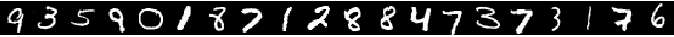
\includegraphics[width = 1.0\textwidth]{normal_mnist.png}
  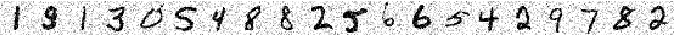
\includegraphics[width = 1.0\textwidth]{noise_inverted_mnist.png}
  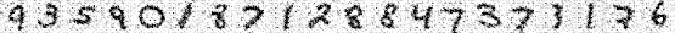
\includegraphics[width = 1.0\textwidth]{noise_reconstruction_mnist.png}
   
\includegraphics[width = 1.0\textwidth]{normal_reconstruction_mnist.png}
     \captionof{figure}{\textbf{First and second row}: Sample of MNIST data set used for training. \textbf{Third and fourth row: Transformed MNIST images.}}
     \label{fig:mnist_data}
     \end{minipage}
  \end{center}
  A GAN was trained to transform the normal images to corrupted images and vice versa. The training procedure is demonstrated in Figure \ref{fig:cycle_diagram}.
  \begin{center}
     \begin{minipage}{\linewidth}
     \centering
   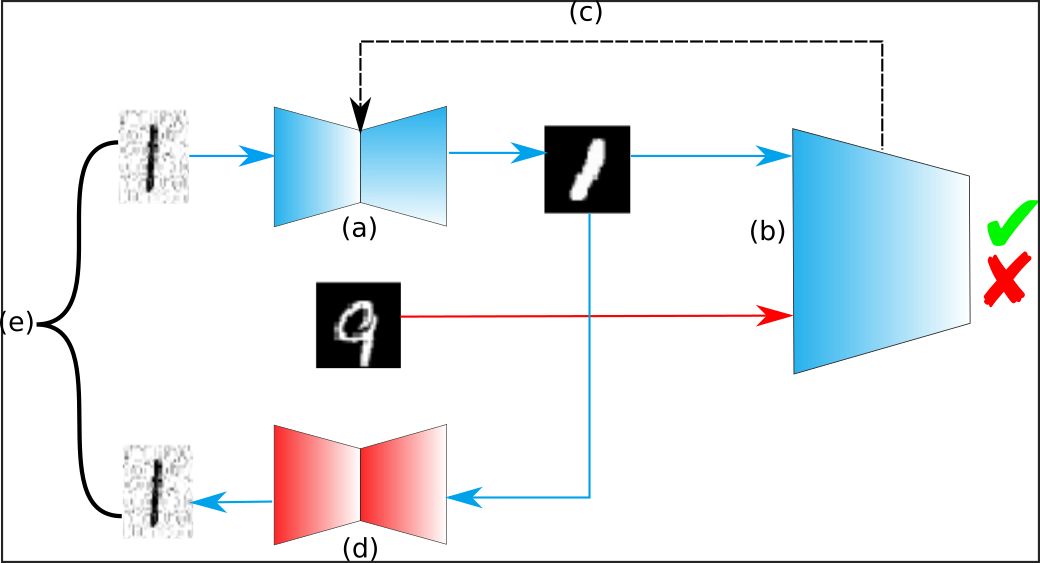
\includegraphics[width = 0.9\textwidth]{cycle_diagram.png}
	\captionof{figure}{}
    \label{fig:cycle_diagram}
     \end{minipage}
  \end{center}
  \textbf{(a)} A generator attempts to transform a corrupted images into a normal image. Since the generator has been initialised with random weights, in the beginning, it produces a random (noisy) image. \textbf{(b)} A discriminator attempts to classify the transformed images as fake and another image from other set as real. The digits do not necessarily have to correspond to each other.
  \textbf{(c)} The classification of the discriminator is used as information to update the generator's parameters. The discriminator, on the other hand, is told which image is fake or real and thus, is trained through supervised learning. \textbf{(d)} Another generator takes transformed image and attempts to reconstruct original image. \textbf{(e)} The original image and reconstructed image is compared and the reconstruction error is used to update both generators' parameters. \textbf{(f)} This process is mirrored for the other set of images using the same respective generators but a different discriminator.

Therefore in each training cycle, the generators undergo two passes, one to transform a real image into a fake image and another to reconstruct a fake image into the original. As training progresses, the generator gradually improves its generation of images in order to fool the discriminator. At convergence, the generator is no longer able to fool the discriminator, and the discriminator is no longer able to distinguish between the observed and generated data.

  The third and fourth row of Figure \ref{fig:mnist_data} show the result of the GAN transformations on an unseen test set. These images demonstrate that the transformation still maintains the input images' most important information, its digit, and at the same time, is able to add characteristics that define the two sets of images. The GAN is able to denoise images (compare the second and bottom row of Figure \ref{fig:mnist_data}) but is also able to deterministically include features that look like Gaussian noise (compare the first row and third row).
  \label{box1:mnist}
  \end{mdframed}
